
%\RequirePackage{pdf15}

\documentclass{beamer}

\usepackage[utf8]{inputenc}

\usepackage{mystyle}

\usepackage{natbib}
\usepackage{tikz}
\usepackage{pgfplots}
\usepackage{multirow}
\usepackage{booktabs}

\usepackage{tikz}
\usepackage{tikz-qtree}
\usetikzlibrary{arrows, shapes.misc, positioning,bayesnet}
\newcommand{\eos}{\texttt{eos}}
\newcommand{\pad}{\texttt{pad}}
\newcommand{\unk}{\texttt{unk}}
\newcommand{\bos}{\texttt{bos}}
%Information to be included in the title page:
\title{Cascaded Text Generation \\ with Markov Transformers}
\author{Anonymous}
\date{2020}

\tikzset{
  invisible/.style={opacity=0},
  visible on/.style={alt={#1{}{invisible}}},
  alt/.code args={<#1>#2#3}{%
    \alt<#1>{\pgfkeysalso{#2}}{\pgfkeysalso{#3}} % \pgfkeysalso doesn't change the path
  },
}

\begin{document}

\frame{\titlepage}

\begin{frame}
\frametitle{Fully Autoregressive vs Nonautoregressive}
\begin{columns}
\begin{column}{0.5\textwidth}
\centering
\only<.(1)->{Fully Autoregressive}
\end{column}
\begin{column}{0.5\textwidth}
\centering
\only<+(12)->{Nonautoregressive {\tiny\citep{gu2017non}}}
\end{column}
\end{columns}
\begin{columns}
\begin{column}{0.5\textwidth}
    \begin{center}
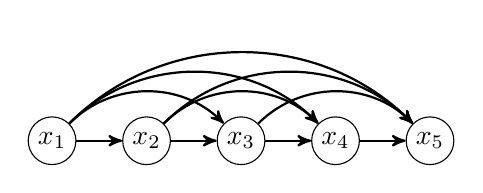
\begin{tikzpicture}[paths/.style={->, thick, >=stealth'}]
\node[shape=circle,draw,inner sep=2pt,minimum size=0pt,visible on=<+(0)->] (x1) at (-2.4,-3) 
     {$x_1$};
 \node[shape=circle,draw,inner sep=2pt,minimum size=0pt,visible on=<+(1)->] (x2) at (-1.2,-3) 
     {$x_2$};
 \node[shape=circle,draw,inner sep=2pt,minimum size=0pt,visible on=<+(2)->] (x3) at (0,-3) 
     {$x_3$};
 \node[shape=circle,draw,inner sep=2pt,minimum size=0pt,visible on=<+(3)->] (x4) at (1.2,-3) 
     {$x_4$};
 \node[shape=circle,draw,inner sep=2pt,minimum size=0pt,visible on=<+(4)->] (x5) at (2.4,-3) 
     {$x_5$};
 
 \draw [paths,visible on=<+(-4)->] (x1) to [] node {} (x2);
 \draw [paths,visible on=<+(-3)->] (x2) to [] node {} (x3);
 \draw [paths,visible on=<+(-2)->] (x3) to [] node {} (x4);
 \draw [paths,visible on=<+(-1)->] (x4) to [] node {} (x5);
 \draw [paths,visible on=<+(-6)->] (x1) to [bend left=45] node {} (x3);
 \draw [paths,visible on=<+(-5)->] (x2) to [bend left=45] node {} (x4);
 \draw [paths,visible on=<+(-4)->] (x3) to [bend left=45] node {} (x5);
 \draw [paths,visible on=<+(-7)->] (x1) to [bend left=45] node {} (x4);
 \draw [paths,visible on=<+(-6)->] (x2) to [bend left=45] node {} (x5);
 \draw [paths,visible on=<+(-7)->] (x1) to [bend left=45] node {} (x5);
 \end{tikzpicture}
\end{center}

\end{column}

\begin{column}{0.5\textwidth}  %%<--- here
     \begin{center}
     \vspace*{1.1cm}
     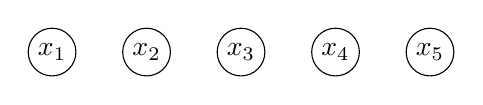
\begin{tikzpicture}[paths/.style={->, thick, >=stealth'}]
\node[shape=circle,draw,inner sep=2pt,minimum size=0pt,visible on=<.(-2)->] (x1) at (-2.4,-3) 
     {$x_1$};
 \node[shape=circle,draw,inner sep=2pt,minimum size=0pt,visible on=<.(-2)->] (x2) at (-1.2,-3) 
     {$x_2$};
 \node[shape=circle,draw,inner sep=2pt,minimum size=0pt,visible on=<.(-2)->] (x3) at (0,-3) 
     {$x_3$};
 \node[shape=circle,draw,inner sep=2pt,minimum size=0pt,visible on=<.(-2)->] (x4) at (1.2,-3) 
     {$x_4$};
 \node[shape=circle,draw,inner sep=2pt,minimum size=0pt,visible on=<.(-2)->] (x5) at (2.4,-3) 
     {$x_5$};
 \end{tikzpicture}
     \end{center}
\end{column}
\end{columns}

\begin{columns}
\begin{column}{0.5\textwidth}
\centering
\begin{itemize}
    \item<+(-6)-> Decoding: beam search
    \item<+(-6)-> Fluent but not serial
\end{itemize}
\end{column}
\begin{column}{0.5\textwidth}
\centering
 \begin{itemize}
     \item<.(-3)-> Decoding: argmax 
     \item<.(-2)-> Parallel but disfluent
 \end{itemize}
\end{column}
\end{columns}
\end{frame}

\begin{frame}
\frametitle{Markov Random Field Framework}
\begin{itemize}
\item {An $m$-th order CRF
\begin{equation*}
    P^{(m)}(x_{1:L}; \theta) \propto \exp \sum_{l=1}^{L-m}f_l^{(m)}(x_{l:l+m}; \theta)
\end{equation*} }
\item<2-> $L=5$, $m=1$
\begin{center}
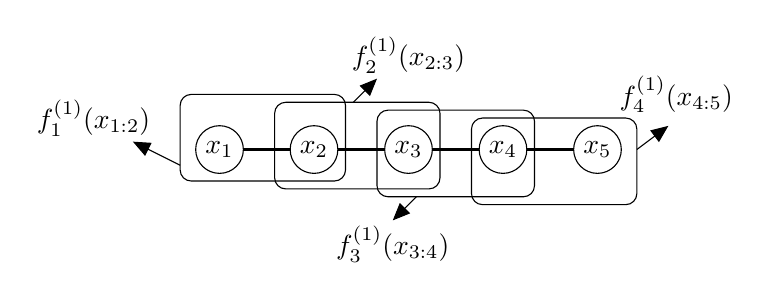
\begin{tikzpicture}[paths/.style={-, thick, >=stealth'}]
\node[shape=circle,draw,inner sep=2pt,minimum size=0pt,visible on=<.(3)->] (x1) at (-2.4,-3) 
     {$x_1$};
 \node[shape=circle,draw,inner sep=2pt,minimum size=0pt,visible on=<.(3)->] (x2) at (-1.2,-3) 
     {$x_2$};
 \node[shape=circle,draw,inner sep=2pt,minimum size=0pt,visible on=<.(3)->] (x3) at (0,-3) 
     {$x_3$};
 \node[shape=circle,draw,inner sep=2pt,minimum size=0pt,visible on=<.(3)->] (x4) at (1.2,-3) 
     {$x_4$};
 \node[shape=circle,draw,inner sep=2pt,minimum size=0pt,visible on=<.(3)->] (x5) at (2.4,-3) 
     {$x_5$};
\node[visible on=<.(4)->] (f1) at (-4.0,-2.6) 
     {$f_1^{(1)}(x_{1:2})$};
     \node[visible on=<.(5)->] (f2) at (0.0,-1.8) 
     {$f_2^{(1)}(x_{2:3})$};
     \node[visible on=<.(6)->] (f3) at (-0.2,-4.2) 
     {$f_3^{(1)}(x_{3:4})$};
     \node[visible on=<.(7)->] (f4) at (3.4,-2.3) 
     {$f_4^{(1)}(x_{4:5})$};
 \draw [paths,visible on=<.(3)->] (x1) to [] node {} (x2);
 \draw [paths,visible on=<.(3)->] (x2) to [] node {} (x3);
 \draw [paths,visible on=<.(3)->] (x3) to [] node {} (x4);
 \draw [paths,visible on=<.(3)->] (x4) to [] node {} (x5);
 \draw[rounded corners,visible on=<.(4)->] (-2.9, -3.4) rectangle (-0.8, -2.3) {};
 \draw [->,visible on=<.(4)->] (-2.9, -3.2) to (-3.5,-2.9);
 \draw[rounded corners,visible on=<.(5)->] (-1.7, -3.5) rectangle (0.4, -2.4) {};
 \draw [->,visible on=<.(5)->] (-0.7, -2.4) to (-0.4,-2.1);
 \draw[rounded corners,visible on=<.(6)->] (-0.4, -3.6) rectangle (1.6, -2.5) {};
 \draw [->,visible on=<.(6)->] (0.1, -3.6) to (-0.2,-3.9);
 \draw[rounded corners,visible on=<.(7)->] (0.8, -3.7) rectangle (2.9, -2.6) {};
 \draw [->,visible on=<.(7)->] (2.9, -3.0) to (3.3,-2.7);
 \end{tikzpicture}
 \end{center}
 \item<7-> Special cases\begin{itemize}
     \item $m=0$: nonautoregressive
     \item $m=L-1$: fully autoregressive
     \item $0<m<L-1$: partially autoregressive
 \end{itemize}
\end{itemize}
\end{frame}


\begin{frame}
\frametitle{How about partially autoregressive?}
\begin{itemize}
\item<+-> {An $m$-th order CRF with $0<m<L-1$}
\item<+-> {Benefits:
\begin{itemize}
    \item Faster than fully autoregressive: Parallel $O(\log L)$ Decoding {\tiny\citep{sarkka2019temporal,rush2020torch}}
    \item More fluent than nonautoregressive: local dependencies
    \item $m$ controls accuracy/speed tradeoff
\end{itemize}
}
\item<+-> Challenge: decoding (Viterbi) takes $O(V^{m+1})$
\begin{itemize}
    \item Vocab size $V$ on the order of $10^4$
    \item Infeasible even for $m=1$
\end{itemize}
\end{itemize}
\end{frame}

\begin{frame}
\frametitle{Cascaded Decoding Algorithm Outline}
Filter the space of all sequences using increasingly higher order models {\tiny\citep{weiss2010structured}}
\begin{enumerate}
\item<+-> Start with $m=0$, only keep $K$ best unigrams at each position
\item<+-> Use $m=1$, keep $K$ best bigrams at each position
\item<+-> Use $m=2$, keep $K$ best trigrams at each position
\item<+-> $\ldots$ until $m=M$ decode (Viterbi) in the filtered space
\end{enumerate}
\end{frame}

\begin{frame}
\frametitle{Cascaded Decoding Illustration}
$L=3$, $K=10$

\begin{enumerate}
    \item<only@1> Start with $m=0$, only keep $K$ best unigrams at each position
    \item<only@2> Use $m=1$, keep $K$ best bigrams at each position
    \item<only@3> Use $m=2$, keep $K$ best trigrams at each position
    \item<only@4> $\ldots$ until $m=M$ decode (Viterbi) in the filtered space
\end{enumerate}
\begin{center}
\begin{overlayarea}{\textwidth}{10cm}
    \only<1>{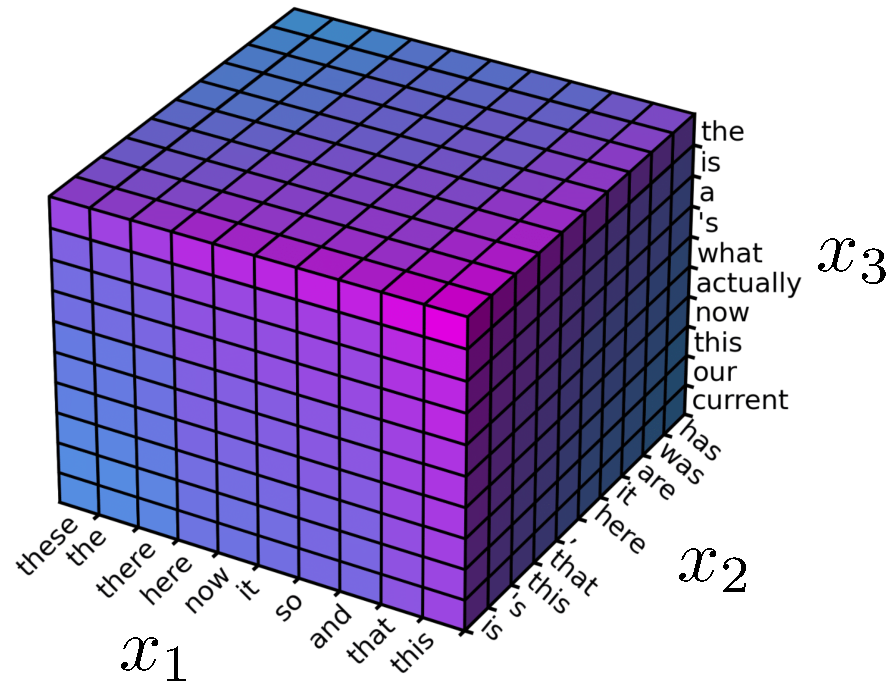
\includegraphics[width=0.8\textwidth]{img/illustration1.pdf}}
    \only<2>{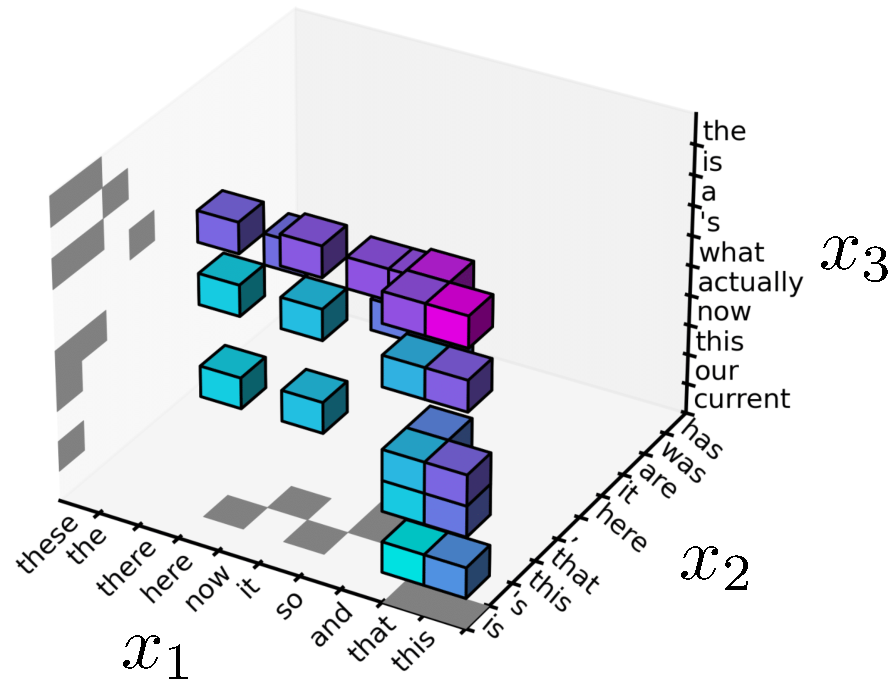
\includegraphics[width=0.8\textwidth]{img/illustration2.pdf}}
    \only<3>{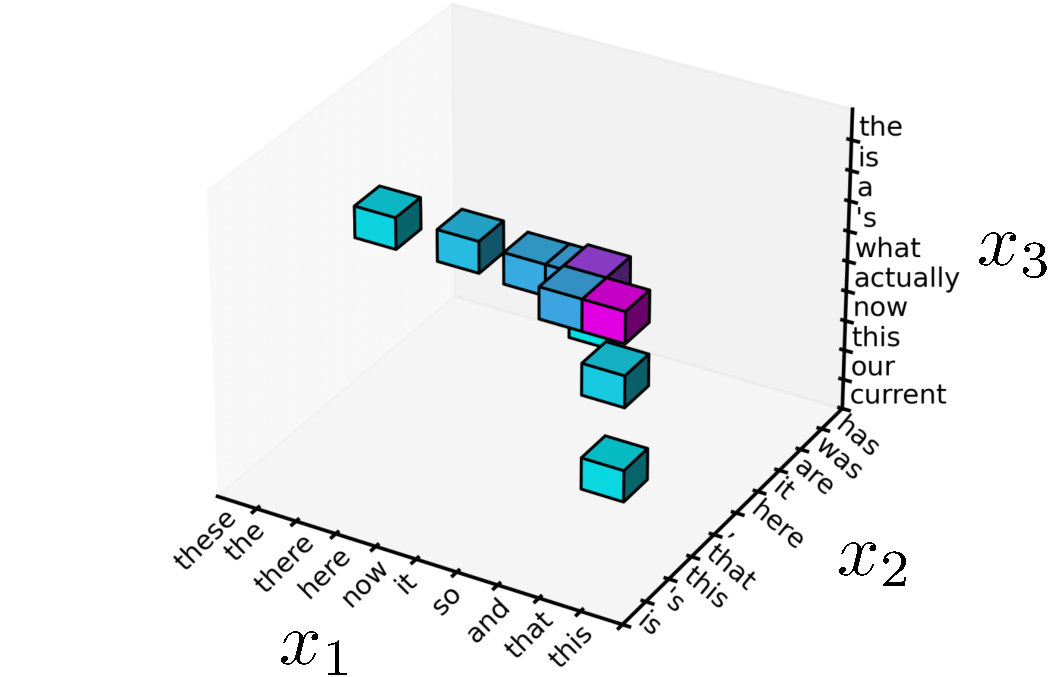
\includegraphics[width=0.8\textwidth]{img/illustration3.pdf}}
    \only<4>{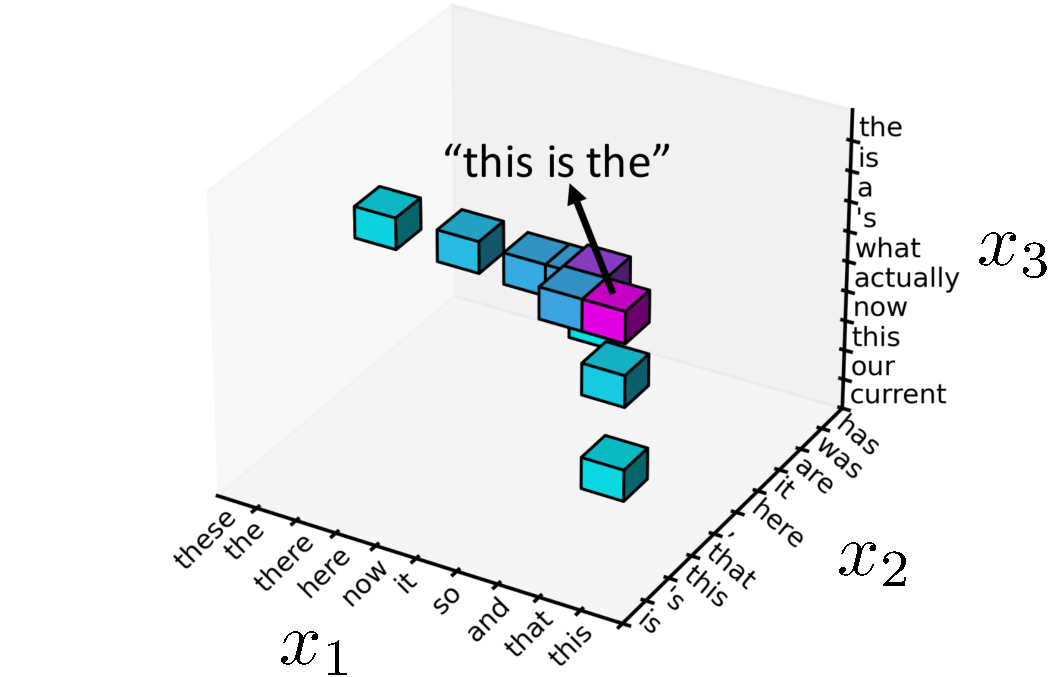
\includegraphics[width=0.8\textwidth]{img/illustration4.pdf}}
\end{overlayarea}
\end{center}
\end{frame}

\begin{frame}
\frametitle{Pruning Criterion}
How to determine the “best” ngrams? Max-marginals.
\begin{itemize}
    \item The max probability of sequences with the given ngram
    \item Directly using ngram potentials cannot consider compatibility with other positions
\end{itemize}
\end{frame}

\begin{frame}
\frametitle{Parallel Decoding (on GPU/TPUs)}
\begin{itemize}
    \item<1-> $f_l^{(m)}$ can be computed in parallel for each position
    \item<2-> Max-marginals can be computed in parallel $O(\log L)$ time
    \item<4-> In practice, as fast as nonautoregressive
    \begin{itemize}
        \item max-marginal takes $<1\%$ total time
    \end{itemize}
\end{itemize}
\begin{center}
     \only<3->{
     \begin{figure}
    \centering
    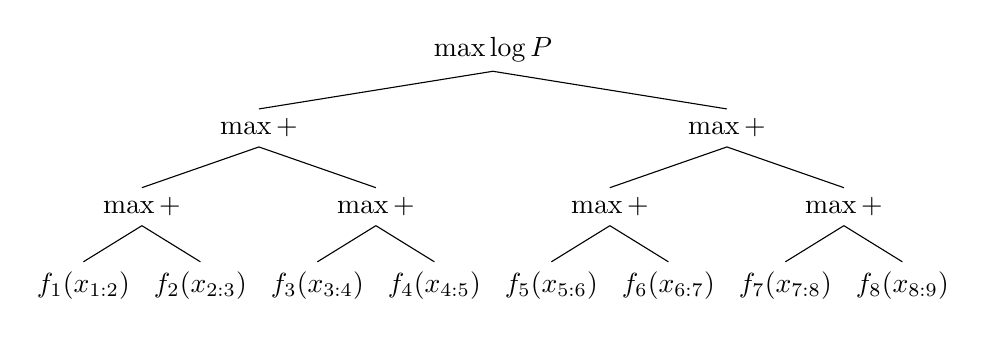
\begin{tikzpicture}[level distance=1cm]
    \Tree [ .$\max \log P$  [ .$\max +$ [.$\max +$ $f_1(x_{1:2})$ $f_2(x_{2:3})$ ] [ .$\max +$ $f_3(x_{3:4})$ $f_{4}(x_{4:5})$ ] ] [.$\max +$  [ .$\max +$ $f_{5}(x_{5:6})$ $f_{6}(x_{6:7})$ ] [ .$\max +$ $f_{7}(x_{7:8})$ $f_8(x_{8:9})$ ] ] ]
    \end{tikzpicture}
\end{figure}
     }
\end{center}
\end{frame}

\begin{frame}
\frametitle{Extension: Variable Length Generation}
\begin{itemize}
    \item<1-> Decoding needs to specify length $L$
    \begin{itemize}
        \item<2-> Same as nonautoregressive approaches
        \item<3-> An inappropriate length limits the best achievable score
    \end{itemize}
    \item<4-> MRF allows considering multiple length values
    \begin{itemize}
        \item<5-> Specify the maximum possible length
        \item<6-> Introduce a special padding symbol
        \item<7-> End-of-sentence/padding always transition to padding
        \item<8-> Trailing paddings do not affect scores
    \end{itemize}
\end{itemize}
\end{frame}

\begin{frame}
\frametitle{A Real Example ($K=5$, max length 8)}
\begin{center}
\vspace{1cm}
    Source: eine erstaunliche frau 
\end{center}
\begin{center}
\begin{overlayarea}{\textwidth}{10cm}
    \only<1>{
    \begin{table}[!htp]
    \centering
    %\caption{\label{tab:amazing}Cascaded Decoding Example. When $m=4$, Viterbi in $\mathcal{X}_4$ returns ``an amazing woman . $\eos$''. The source is ``eine erstaunliche frau . $\eos$'' and the target is ``an amazing woman . $\eos$''.}
       \fontsize{6.5pt}{7.2pt}
       \selectfont
    \begin{tabular}{@{ }l@{ }l@{ }l@{ }l@{ }l@{ }l@{ }l@{ }l@{ }l@{ }l@{ }l@{ }l@{ }l@{ }l@{ }l@{ }l@{ }l@{ }l@{ }l@{ }l@{ }l@{}}
    \toprule
   $m$ & $x_{1:1+m}$ & $x_{2:2+m}$ & $x_{3:3+m}$ & $x_{4:4+m}$ & $x_{5:5+m}$ & $x_{6:6+m}$ &$x_{7:7+m}$ & $x_{8}$\\
            \midrule
    \multirow{5}{*}{0}   & an           &amazing    & woman     & woman     & $\eos$    & $\eos$    & $\eos$    & $\pad$ \\
                        & amazing       &woman      & amazing   & .         & .         & $\pad$    & $\pad$    & -\\
                        & incredible    &an         & an        & amazing   & woman     & .         & .         & - \\
                        &this           &remarkable & .         & $\eos$    & amazing   & woman     & woman     & -  \\
                        &remarkable     &incredible & women     & an        & women     & women     & women     & - \\
    \bottomrule
    \end{tabular}
\end{table}
    }
    \only<2>{
    \begin{table}[!htp]
    \centering
    %\caption{\label{tab:amazing}Cascaded Decoding Example. When $m=4$, Viterbi in $\mathcal{X}_4$ returns ``an amazing woman . $\eos$''. The source is ``eine erstaunliche frau . $\eos$'' and the target is ``an amazing woman . $\eos$''.}
       \fontsize{6.5pt}{7.2pt}
       \selectfont
    \begin{tabular}{@{ }l@{ }l@{ }l@{ }l@{ }l@{ }l@{ }l@{ }l@{ }l@{ }l@{ }l@{ }l@{ }l@{ }l@{ }l@{ }l@{ }l@{ }l@{ }l@{ }l@{ }l@{}}
    \toprule
   $m$ & $x_{1:1+m}$ & $x_{2:2+m}$ & $x_{3:3+m}$ & $x_{4:4+m}$ & $x_{5:5+m}$ & $x_{6:6+m}$ &$x_{7:7+m}$ \\
            \midrule
    \multirow{5}{*}{1}   & an  amazing         &amazing woman    & woman .              & . $\eos$      & $\eos$ $\pad$ & $\pad$ $\pad$    & $\pad$ $\pad$\\
                        & an incredible       &incredible woman      & amazing woman          & woman .       & . $\eos$      & $\eos$ $\pad$    & $\eos$ $\pad$ \\
                        & this amazing    &remarkable woman         & women .             & amazing woman & woman .       & .  $\eos$       & -  \\
                        &an remarkable           &woman amazing & woman woman             & . .           & women .       & woman $\eos$     & -\\
                        &amazing woman     &amazing women      & an amazing        & . woman       & . .     & -      &        -   &\\
    \bottomrule
    \end{tabular}
\end{table}
    }
    \only<3>{
    \begin{table}[!htp]
    \centering
    %\caption{\label{tab:amazing}Cascaded Decoding Example. When $m=4$, Viterbi in $\mathcal{X}_4$ returns ``an amazing woman . $\eos$''. The source is ``eine erstaunliche frau . $\eos$'' and the target is ``an amazing woman . $\eos$''.}
       \fontsize{6.5pt}{7.2pt}
       \selectfont
    \begin{tabular}{@{ }l@{ }l@{ }l@{ }l@{ }l@{ }l@{ }l@{ }l@{ }l@{ }l@{ }l@{ }l@{ }l@{ }l@{ }l@{ }l@{ }l@{ }l@{ }l@{ }l@{ }l@{}}
    \toprule
   $m$ & $x_{1:1+m}$ & $x_{2:2+m}$ & $x_{3:3+m}$ & $x_{4:4+m}$ & $x_{5:5+m}$ & $x_{6:6+m}$  \\
            \midrule
    \multirow{5}{*}{2}   & an amazing woman         &amazing woman .   & woman .$\eos$& . $\eos$ $\pad$     & $\eos$ $\pad$ $\pad$ & $\pad$ $\pad$ $\pad$\\
                        & an incredible woman      &incredible woman .     & women . $\eos$         & woman . $\eos$      & . $\eos$  $\pad$     & $\eos$ $\pad$ $\pad$ \\
                        & this amazing woman    &remarkable woman .        & woman woman .            & . . $\eos$ & woman .  $\eos$          & .  $\eos$ $\pad$ \\
                        &an remarkable woman           &amazing women . & woman . .             & . woman .         & . . $\eos$     & -   \\
                        &an amazing women     &amazing woman woman      & woman . woman       & woman . .     & -       &  -       &\\
    \bottomrule
    \end{tabular}
\end{table}
    }
    \only<4>{
    \begin{table}[!htp]
    \centering
    %\caption{\label{tab:amazing}Cascaded Decoding Example. When $m=4$, Viterbi in $\mathcal{X}_4$ returns ``an amazing woman . $\eos$''. The source is ``eine erstaunliche frau . $\eos$'' and the target is ``an amazing woman . $\eos$''.}
       \fontsize{6.5pt}{7.2pt}
       \selectfont
    \begin{tabular}{@{ }l@{ }l@{ }l@{ }l@{ }l@{ }l@{ }l@{ }l@{ }l@{ }l@{ }l@{ }l@{ }l@{ }l@{ }l@{ }l@{ }l@{ }l@{ }l@{ }l@{ }l@{}}
    \toprule
   $m$ & $x_{1:1+m}$ & $x_{2:2+m}$ & $x_{3:3+m}$ & $x_{4:4+m}$ & $x_{5:5+m}$ \\
            \midrule
    \multirow{5}{*}{3}   & an amazing woman .        &amazing woman . $\eos$   & woman . $\eos$ $\pad$         & . $\eos$ $\pad$ $\pad$     & $\eos$ $\pad$ $\pad$ $\pad$ \\
                        & an incredible woman .     &incredible woman . $\eos$     & women . $\eos$ $\pad$        & woman . $\eos$ $\pad$     & . $\eos$ $\pad$ $\pad$   \\
                        & this amazing woman .   &remarkable woman . $\eos$       & woman woman . $\eos$            &. . $\eos$ $\pad$ &woman . $\eos$ $\pad$    \\
                        &an remarkable woman .          &amazing women . $\eos$ & woman . . $\eos$            & . woman . $\eos$       & . . $\eos$ $\pad$      & \\
                        &an amazing women .    &amazing woman woman .     & woman . woman .      &woman . . $\eos$    & -            &\\
    \bottomrule
    \end{tabular}
\end{table}
    }
    \only<5>{\centering Viterbi Result: ``an amazing woman . $\eos$''}
\end{overlayarea}
\end{center}
\end{frame}

\begin{frame}
\frametitle{Modeling Support: Markov Transformer}
\begin{center}
    \only<2->{How to get different models of different orders $m$?}
\end{center}
\begin{itemize}
    \item<3-> Training: reset the hidden state every $M$ words
    \item<5-> Test: a single Markov transformer can be used as any $m<M$ order model
\end{itemize}

\begin{columns}
\begin{column}{0.68\textwidth}
\centering
\only<4->{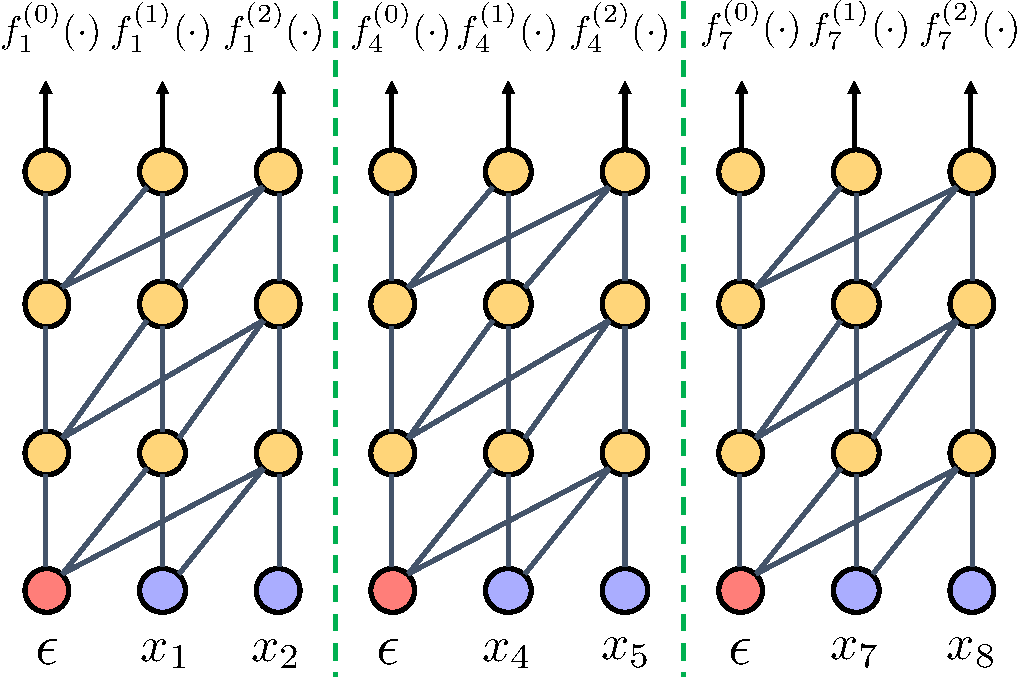
\includegraphics[width=\textwidth]{img/markov_train_new.pdf}}
\end{column}
\begin{column}{0.27\textwidth}
\centering
\only<6->{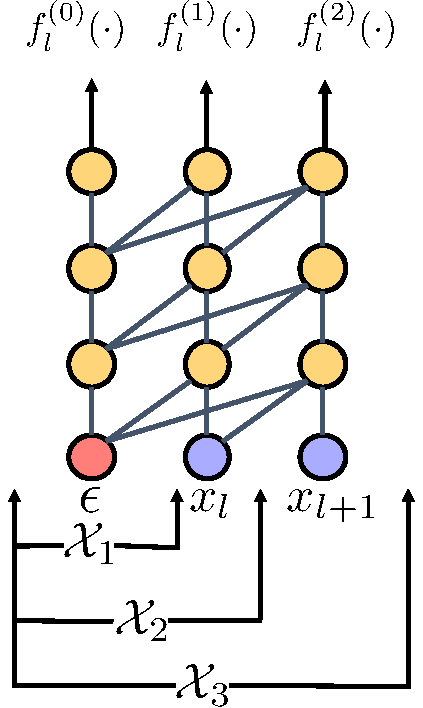
\includegraphics[width=\textwidth]{img/markov_cascade_new.pdf}}
\end{column}
\end{columns}

\end{frame}

\begin{frame}
\frametitle{Results I: Speed/Accuracy Tradeoff}
\begin{itemize}
    \item Translation on IWSLT (w/ distillation {\tiny\citep{kim2016sequence}})
\end{itemize}

\begin{table}[H]
    \centering
    %\caption{\label{tab:main-5} Results on IWSLT14 De-En.}
    %\scriptsize
    \begin{tabular}{@{}l@{}lr@{ }lccccccc@{}}
    \toprule
       \ \  Model     &  Settings                  &       \multicolumn{2}{c}{Latency (Speedup)}                & BLEU   \\
    \midrule
    %\emph{Fully Autoregressive}\\229.76
    \ \ Transformer &(beam 5)  &229.76ms & ($\times1.00$)         &         34.44           \\
    \midrule
    %\textbf{With Distillation}\\
    Cascaded Generation &\hspace{0.01cm} \emph{with Speedup}\\
    \ \ $> \times 6/5$ &(K=16, iters=2)&39.38ms & ($\times5.83$)       &  33.90 \\
%\ \ $> \times 6/5$ &(K=16, iters=2)&43.41ms & ($\times6.79$)       &  30.69 \\
%\ \ $> \times 6/5$& (K=32, iters=2)&52.93ms &($\times6.02$)       &  30.72  \\
\ \ $> \times 4$ &(K=32, iters=3)&60.27ms& ($\times3.81$)        & 34.33  \\
%\ \  $\text{Val Speedup}>3$ (K=32, rounds=3)&N& 26.77 & 80.1ms (3.98) & 31.08 &       & 33.16 & 33.12 &       & 34.33 \\
\ \ $> \times 3$ &(K=32, iters=4)&78.27ms &($\times2.94$)       &  34.43 \\
%\ \ $\text{Val Speedup}>2$ (K=64, rounds=4)&N& 26.90 & 150.61ms (2.12)       & 31.28 &       & 33.30 & 33.29 &       & 34.55 \\
\ \ $>\times 2/1$ &(K=64, iters=5)&117.90ms &($\times1.95$)       &  34.49 \\
%\ \ Barrier + Cascade (K=16, rounds=2)&N& 26.34 & 50.28ms (6.34)        & 30.69 & 43.41ms (6.79)        &       & 32.70 & 49.38ms (6.95)        & 32.66 & 46.84ms (6.8) &       & 33.90 & 39.38ms (5.83)        \\
%\ \ Barrier + Cascade (K=16, rounds=3)&N& 26.60 & 67.49ms (4.72)        & 30.96 & 62.06ms (4.75)        &       & 32.89 & 66.33ms (5.18)        & 33.00 & 62.57ms (5.09)        &       & 34.19 & 53.1ms (4.33) \\
%\ \ Barrier + Cascade (K=16, rounds=4)&N& 26.73 & 92.3ms (3.45) & 31.11 & 82.41ms (3.58)        &       & 32.92 & 78.82ms (4.36)        & 33.08 & 80.5ms (3.96) &       & 34.29 & 69.96ms (3.28)        \\
%\ \ Barrier + Cascade (K=16, rounds=5)&N& 26.68 & 104.84ms (3.04)       & 31.03 & 101.67ms (2.9)        &       & 32.86 & 95.06ms (3.61)        & 33.04 & 99.25ms (3.21)        &       & 34.30 & 83.93ms (2.74)        \\
%\ \ Barrier + Cascade (K=32, rounds=2)&N& 26.43 & 52.93ms (6.02)        & 30.72 & 52.06ms (5.66)        &       & 32.73 & 54.56ms (6.29)        & 32.70 & 54.26ms (5.87)        &       & 34.01 & 41.09ms (5.59)        \\
%\ \ Barrier + Cascade (K=32, rounds=3)&N& 26.77 & 80.1ms (3.98) & 31.08 & 79.01ms (3.73)        &       & 33.16 & 77.39ms (4.44)        & 33.12 & 75.95ms (4.19)        &       & 34.33 & 60.27ms (3.81)        \\
%\ \ Barrier + Cascade (K=32, rounds=4)&N& 26.80 & 107.14ms (2.98)       & 31.22 & 107.71ms (2.74)       &       & 33.14 & 97.14ms (3.53)        & 33.22 & 100.17ms (3.18)       &       & 34.43 & 78.27ms (2.94)        \\
%\ \ Barrier + Cascade (K=32, rounds=5)&N& 26.90 & 132.64ms (2.4)        & 31.15 & 129.67ms (2.27)       &       & 33.08 & 118.89ms (2.89)       & 33.13 & 123.05ms (2.59)       &       & 34.43 & 96.71ms (2.38)        \\
%\ \ Barrier + Cascade (K=64, rounds=2)&N& 26.52 & 68.09ms (4.68)        & 30.73 & 66.85ms (4.41)        &       & 32.77 & 66.59ms (5.16)        & 32.76 & 68.02ms (4.68)        &       & 34.02 & 48.28ms (4.76)        \\
%\ \ Barrier + Cascade (K=64, rounds=3)&N& 26.88 & 111.22ms (2.87)       & 31.17 & 109.4ms (2.69)        &       & 33.23 & 108.57ms (3.16)       & 33.17 & 103.85ms (3.07)       &       & 34.46 & 74.12ms (3.1) \\
%\ \ Barrier + Cascade (K=64, rounds=4)&N& 26.90 & 150.61ms (2.12)       & 31.28 & 150.6ms (1.96)        &       & 33.30 & 142.23ms (2.41)       & 33.29 & 146.86ms (2.17)       &       & 34.55 & 99.22ms (2.32)        \\
%\ \ Barrier + Cascade (K=64, rounds=5)&N& 26.92 & 189.96ms (1.68)       & 31.23 & 187.56ms (1.57)       &       & 33.23 & 179.07ms (1.92)       & 33.28 & 181.18ms (1.76)       &       & 34.49 & 117.9ms (1.95)        \\
%\ \ Barrier + Cascade (K=128, rounds=2)&N& 26.54        & 115.52ms (2.76)       & 30.81 & 113.69ms (2.59)       &       & 32.66 & 113.95ms (3.01)       & 32.83 & 112.55ms (2.83)       &       & 34.05 & 73.96ms (3.11)        \\
%\ \ Barrier + Cascade (K=128, rounds=3)&N& 26.96        & 192.19ms (1.66)       & 31.16 & 188.17ms (1.57)       &       &       &       &       &       & 34.50 & 110.55ms (2.08)       \\
%\ \ Barrier + Cascade (K=128, rounds=4)&N& 27.01        & 266.95ms (1.19)       & 31.23 & 261.89ms (1.13)       &       &       &       &       &       & 34.57 & 146.48ms (1.57)       \\
%\ \ Barrier + Cascade (K=128, rounds=5)&N& 27.04        & 337.54ms (0.94)       & 31.20 & 331.67ms (0.89)       &       &       &       &       &       & 34.52 & 180.17ms (1.28)       \\
 %    \midrule
 %     \textbf{Without Distillation}\\
 %     Cascaded Generation & \hspace{0.01cm} \emph{with Speedup}\\
%\ \ $>\times 5$ & (K=64, iters=2)&48.59ms &($\times4.73$)        & 33.25  \\
%\ \ $>\times 4$ &(K=64, iters=2)&69.19ms &($\times4.61$)&           27.79 \\
%\ \ $>\times 3$ &(K=64, iters=3)&75.64ms& ($\times3.04$)        & 33.96 \\
%\ \ $>\times 2$ &(K=64, iters=5)&121.95ms &($\times1.88$)       & 34.08  \\
%\ \ $>\times 1$ &(K=128, iters=5)&189.10ms &($\times1.22$)       &  34.15 \\
    \bottomrule
    \end{tabular}
\end{table}

\end{frame}

\begin{frame}
\frametitle{Results II: Number of Sequences Scored}
\begin{itemize}
    \item<1-> Beam search only scores $KL$ full sequences
    \item<2-> Cascaded Search can score exponential number of sequences
\end{itemize}
\begin{center}
    \only<3->{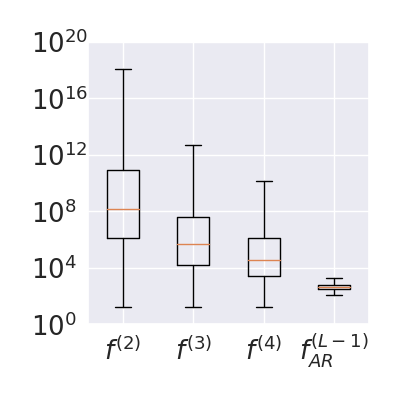
\includegraphics[width=0.7\textwidth]{img/count_paper_nogt_latest.png}}
\end{center}
\end{frame}

\begin{frame}
\frametitle{Conclusions}
\begin{itemize}
    \item<1-> Nonautoregressiveness is sufficient but unnecessary for fast text generation
    \item<2-> MRF model with a fixed order
    \begin{itemize}
        \item Faster than fully autoregressive
        \item More fluent than nonautoregressive
    \end{itemize}
\item<3-> Cascaded search efficiently decodes a fixed order MRF
\item<4-> Markov transformer makes a single model usable as a cascade
\end{itemize}
\end{frame}




\begin{frame}
\frametitle{Citations}
\bibliographystyle{acl_natbib}
\bibliography{anthology,emnlp2020}
\end{frame}


\end{document}
